\chapter[Random Variables]{Random Variables}
\section{Random Variables: Examples and Definitions}
In practical applications we are typically interested in numerical features associated to an outcome of an experiment. 

\begin{ex}
    Suppose we toss a two sided coin three times. The sample space of this experiment is given by: 
    $$\mathcal{S} := \begin{Bmatrix}
         HHH, & HHT, & HTT, &TTT  \\
            & HTH, & THT,& \\
            &THH, & TTH&
    \end{Bmatrix}
    $$
    We can consider numerical features of an outcome in the sample space, for example:
    \begin{enumerate}
        \item How many heads in the outcome?
        \item How many tails in the outcome?
        \item Are there more heads than tails?
        \item Is the first toss in the outcome a head?
        \item Is the last toss a tails?
        \item How many tails till the first head?
    \end{enumerate}
\end{ex}

\begin{ex}
    Suppose we randomly sample a student from the campus. The sample space for this experiment is given by:
    $$\mathcal{S} : = \{ \text{All students on campus}\}$$
    We can consider numerical features of an outcome (a student from the campus) in the sample space, for example:
    \begin{enumerate}
        \item What is the height of the chosen student?
        \item What is the average daily commute time for the student?
        \item The number of credits the student is enrolled in?
        \item The number of electronic gadgets the student owns?
        \item Average number of people the student interacts with on a given day?
        \item Is the student an athlete?
    \end{enumerate}
\end{ex}
These questions provide answers to very specific numeric/quantitative features of the student. 

\begin{defn}[Random Variable]
    A random variable $X$ is a real valued function on the sample space $\mathcal{S}$. That is, 
    \begin{eqnarray*}
        X :& \mathcal{S} &\longrightarrow \mathbb{R}\\
        & \omega &\mapsto X(\omega)
    \end{eqnarray*}
    The range of $X$, that is the set of all possible values that $X$ can take will be denoted as $\mathcal{X}$
\end{defn}
Intuitively, a random variable measures a specific quantitative feature of the sample space outcome. Here is a schematic to consider: 
\begin{center}
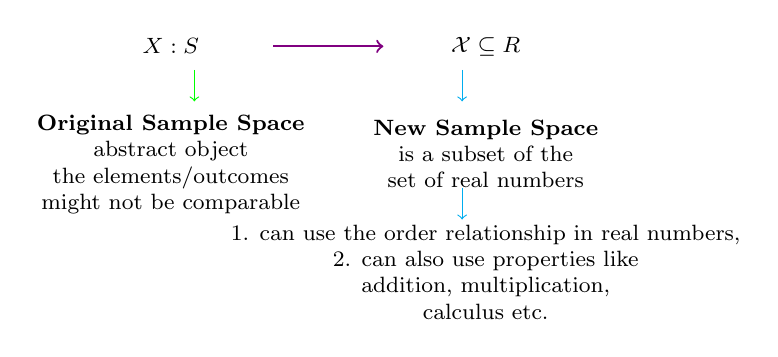
\begin{tikzpicture}
\tikzset{every node/.style={font=\footnotesize}}

% Function arrow and labels
\node at (-1.5, 0) (domain) {$X : S$};
\node at (2.5, 0) (codomain) {$\mathcal{X} \subseteq \mathbb{R}$};
\draw[->, thick, violet] (-0.2, 0) -- (1.2, 0);

% Left note
\node at (-1.5, -1.5) [align=center] {\textbf{Original Sample Space} \\ abstract object \\ the elements/outcomes \\ might not be comparable};

% Right note
\node at (2.5, -2.2) [align=center] {\textbf{New Sample Space} \\ is a subset of the \\ set of real numbers \\ \\ 1. can use the order relationship in real numbers, \\ 2. can also use properties like \\ addition, multiplication, \\ calculus etc.};

% Braces

% Arrows from notes to labels
\draw[->,green] (-1.2, -0.3) -- (-1.2, -0.7);
\draw[->,cyan] (2.2, -0.3) -- (2.2, -0.7);
\draw[->,cyan] (2.2, -1.8) -- (2.2, -2.2);

\end{tikzpicture}
\end{center}

\begin{defn}[Events Associated to a Random Variable]
    Given a random variable $$X: \mathcal{S} \longrightarrow \mathbb{R}$$
    we can use the order relationship of $\mathbb{R}$ to consider the following "interesting events" for $X$:
    \begin{eqnarray*}
        \{a \le X \le b\} :=& \text{$X$ takes values in the interval $[a, b]$}\\
        \{a \le X \} :=& \text{$X$ takes values in the interval $[a, \infty)$}\\
        \{ X \le b\} :=& \text{$X$ takes values in the interval $[-\infty, b]$}\\
    \end{eqnarray*}
    We can also allow for strict inequalities, countable unions, complements, and countable intersections. 
    \\
    We will assume that we are able to calculate the probabilities associated to these events, and these will be denoted by $P(a\le X \le b), P(a \le X), P(X \le b)$, etc
\end{defn}


\begin{ex}Suppose the sample space $\mathcal{S}$ is all students on campus.

For $ \omega \in \mathcal{S}$, we define:
\[
X(\omega) := \text{height of } \omega \text{ (in inches)}
\]

What are the values of \( X \)?

\[
\mathcal{X} := (0, \infty)
\]

Some "interesting events" corresponding to $X$ can be:
\begin{eqnarray*}
    \{ 60 \leq X \leq 65 \} &:=& \{ \omega \in S \mid X(\omega) \in [60, 65] \}\\
&=& \{\text{set of all students whose height is between 60 and 65 inches.}\}
\end{eqnarray*}

\begin{eqnarray*}
    \{X \ge 72\} &:=& \{ \omega \in S \mid X(\omega) \in [72, \infty) \}\\
    &=&\{\text{all students whose height is greater than or equal to 72 inches}\} 
\end{eqnarray*}

    
\end{ex}
%%%%%%%%%%%%%%%%%%%% Example: toss a coin three times %%%%%%%%%%%%%%%%
\begin{ex}
Suppose we toss a coin three times, and we want to know if the first toss was a head?
    \begin{equation*}
    X(\omega) =
    \begin{cases}
    0 & \text{if first toss in } \omega \text{ is not H} \\
    1 & \text{otherwise}
    \end{cases}
    \end{equation*}


\begin{center}
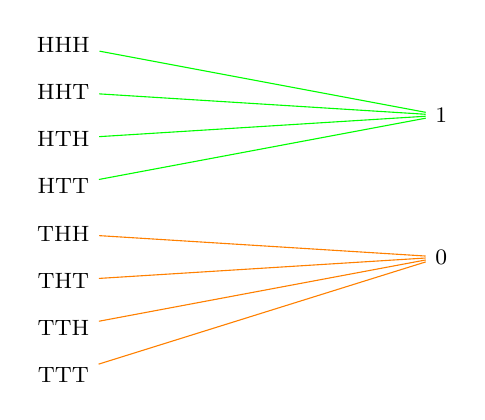
\begin{tikzpicture}[scale=1.2]
\tikzset{every node/.style={font=\footnotesize}}

% Nodes for outcomes
\node at (0, 4) (HHH) {HHH};
\node at (0, 3.5) (HHT) {HHT};
\node at (0, 3) (HTH) {HTH};
\node at (0, 2.5) (HTT) {HTT};
\node at (0, 2) (THH) {THH};
\node at (0, 1.5) (THT) {THT};
\node at (0, 1) (TTH) {TTH};
\node at (0, 0.5) (TTT) {TTT};

% Nodes for outputs
\node at (4, 3.25) (1) {1};
\node at (4, 1.75) (0) {0};



% Lines for 0
\draw[green] (HHH) -- (1);
\draw[green] (HHT) -- (1);
\draw[green] (HTH) -- (1);
\draw[green] (HTT) -- (1);

% Lines for 1
\draw[orange] (THH) -- (0);
\draw[orange] (THT) -- (0);
\draw[orange] (TTH) -- (0);
\draw[orange] (TTT) -- (0);
\end{tikzpicture}
\end{center}

Another way of looking at it:
\begin{equation*}
\begin{aligned}
    \{ X = 0 \} := X^{-1}(0) & = \{ \text{all sample space outcomes on which } X \text{ takes value 0} \} \\
    & = \{ \text{THH, THT, TTH, TTT} \}
\end{aligned}
\end{equation*}
Similarly,
\begin{equation*}
\begin{aligned}
    & \{ X = 1 \} := X^{-1}(1) = \{ \text{HHH, HTH, HHT, HTT} \}
\end{aligned}
\end{equation*}

\begin{equation*}
\begin{aligned}
    S := \{ & \{ \text{HHH, HTH, HHT, HTT} \} \mapsto \{1\}, \{ \text{THH, THT, TTH, TTT} \} \mapsto \{ 0 \} \}
\end{aligned}
\end{equation*}

\end{ex}


\begin{ex} 
Suppose we tossed a coin three times, and we were interested in counting the number of heads in three tosses. We can work through this as follows:

\begin{equation*}
X(\omega) := \# \text{ of heads in three tosses.}
\end{equation*}

\begin{center}
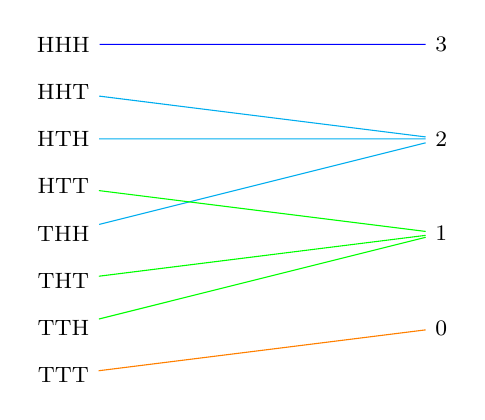
\begin{tikzpicture}[scale=1.2]
\tikzset{every node/.style={font=\footnotesize}}

% Nodes for outcomes
\node at (0, 4) (HHH) {HHH};
\node at (0, 3.5) (HHT) {HHT};
\node at (0, 3) (HTH) {HTH};
\node at (0, 2.5) (HTT) {HTT};
\node at (0, 2) (THH) {THH};
\node at (0, 1.5) (THT) {THT};
\node at (0, 1) (TTH) {TTH};
\node at (0, 0.5) (TTT) {TTT};

% Nodes for outputs
\node at (4, 4) (3) {3};
\node at (4, 3) (2) {2};
\node at (4, 2) (1) {1};
\node at (4, 1) (0) {0};




% Lines for 3
\draw[blue] (HHH) -- (3);

% Lines for 2
\draw[cyan] (HHT) -- (2);
\draw[cyan] (HTH) -- (2);
\draw[cyan] (THH) -- (2);

% Lines for 1
\draw[green] (THT) -- (1);
\draw[green] (HTT) -- (1);
\draw[green] (TTH) -- (1);

% Lines for 0
\draw[orange] (TTT) -- (0);
\end{tikzpicture}
\end{center}

\begin{equation*}
\begin{aligned}
    & \{ X = 0 \} = \{ \text{TTT} \} \\
    & \{ X = 1 \} = \{ \text{HTT, THT, TTH} \} \\
    & \{ X = 2 \} = \{ \text{HHT, HTH, THH} \} \\
    & \{ X = 3 \} = \{ \text{HHH} \}
\end{aligned}
\end{equation*}

\begin{equation*}
\mathcal{S} = \left\{
\begin{aligned}
    & \{ \text{HHH} \} \quad && \mapsto 3 \\[4pt]
    & \{ \text{HHT, HTH, THH} \} \quad && \mapsto 2 \\[4pt]
    & \{ \text{HTT, THT, TTH} \} \quad && \mapsto 1 \\[4pt]
    & \{ \text{TTT} \} \quad && \mapsto 0 
\end{aligned} 
\right\}
\end{equation*}

\begin{center}
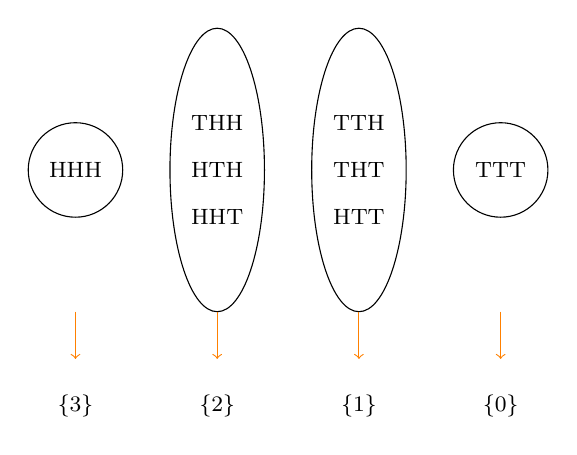
\begin{tikzpicture}[scale=1.2]
\tikzset{every node/.style={font=\footnotesize}}

% Ellipses and elements inside
\draw (0,0) ellipse (0.5cm and 0.5cm);
\draw (1.5,0) ellipse (0.5cm and 1.5cm);
\draw (3,0) ellipse (0.5cm and 1.5cm);
\draw (4.5,0) ellipse (0.5cm and 0.5cm);

\node at (0, 0) {HHH};

\node at (1.5, -0.5) {HHT};
\node at (1.5, 0) {HTH};
\node at (1.5, 0.5) {THH};

\node at (3, -0.5) {HTT};
\node at (3, 0) {THT};
\node at (3, 0.5) {TTH};

\node at (4.5, 0) {TTT};

%\node at (-1, 0) {$\mathcal{S} = \left\{ \right.$}; % Big left curly brace
%\node at (5.5, 0) {$\left. \right\}$}; % Big right curly brace

\node at (0, -2.5) {\{3\}};
\node at (1.5, -2.5) {\{2\}};
\node at (3, -2.5) {\{1\}};
\node at (4.5, -2.5) {\{0\}};

% Arrows
\draw[->,orange] (0, -1.5) -- (0, -2);
\draw[->,orange] (1.5, -1.5) -- (1.5, -2);
\draw[->,orange] (3, -1.5) -- (3, -2);
\draw[->,orange] (4.5, -1.5) -- (4.5, -2);

\end{tikzpicture}
\end{center}
\end{ex}
%%%%%%%%%%%%%%%%%%%%%%%%% end of example %%%%%%%%%%%%%%




\begin{defn}[Cumulative Distribution Function]
    The cummulative distribution function associated to a random variable $$X: \mathcal{S} \longrightarrow \mathbb{R}$$
    is defined as 
    \begin{eqnarray*}
        F_X :& \mathbb{R} &\longrightarrow \mathbb{R}\\
        & x &\mapsto P(X \le x)
    \end{eqnarray*}
    that is
    \begin{eqnarray*}
        F_X(x) := P(\text{$X$ takes values less than or equal to $x$}) 
    \end{eqnarray*}
\end{defn}

%%%%% Example: Toss a coin once 
\begin{ex}
    Suppose we toss a coin with $P(H) = p \in (0,1)$ once. Let $X$ be the random variable that tracks the outcome of the coint toss, that is 
    $$X(\omega) = \begin{cases}
        1 \quad \text{if $\omega = H$}\\
        0 \quad \text{if $\omega = T$}
    \end{cases}$$
    We now calculate the cumulative distribution function for $X$. 

    \begin{enumerate}
        \item If $x < 0$:
\begin{eqnarray*}
\{X \leq x\} &=& \{\text{event that is impossible}\} \\
&=& \emptyset \\
\end{eqnarray*}
Therefore we must have:
\begin{eqnarray*}
    F_X(x) &=& P(X \leq x)\\
    &=& P(\emptyset) \\
    &=& 0
\end{eqnarray*}
for all $x <0$. 
\item If $x = 0$, 
\begin{eqnarray*}
    F_X(0) &=&  P(X \leq 0) \\
&=& \underbrace{P(X < 0)}_{0} + \underbrace{P(X = 0)}_{P(T)=(1-p)} 
\end{eqnarray*}
Therefore,
$$F_X(0) = 1-p$$
\item If $x \in (0,1)$,
\begin{eqnarray*}
    F_X(x) &=& P(X \leq x) \\
&=& \underbrace{P(X \leq 0)}_{0} + \underbrace{P(X=0)}_{1-p} + \underbrace{P(0<X<x<1)}_{0} \\
\end{eqnarray*}
Therefore, 
$$F_X(x) = (1-p) \quad \text{for all } x \in (0,1)$$
\item If $x=1$, 
\begin{eqnarray*}
    F_X(1) &=&  P(X \leq 1) \\
&=& \underbrace{P(X < 1)}_{1-p} + \underbrace{P(X = 1)}_{P(H)=p} 
\end{eqnarray*}
Therefore, 
$$F_X(1) = 1 $$
\item If $x>1$, 
\begin{eqnarray*}
    F_X(x) &=&  P(X \leq x) \\
&=& \underbrace{P(X \le 1)}_{1} + \underbrace{P(X > 1)}_{0} 
\end{eqnarray*}
Therefore, 
$$F_X(x) = 1 \quad \text{for all } x > 1 $$

    \end{enumerate}



The cdf $F_X$ can be written as follows:

\[
F_X(x) = \begin{cases}
0 & \text{if } x < 0 \\
(1-p) & \text{if } x \in [0,1) \\
1 & \text{if } x \geq 1
\end{cases}
\]

The plot of $F_X(x)$:
\vspace{1em}

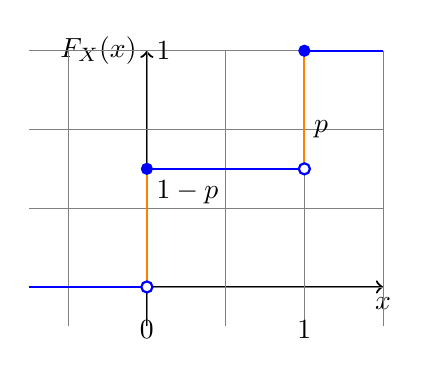
\begin{tikzpicture}
    % Axis
    \draw[thick, ->] (-1.5,0) -- (3,0) node[anchor=north] {$x$};
    \draw[thick, ->] (0,-0.5) -- (0,3) node[anchor=east] {$F_X(x)$};
    \draw[very thin, gray] (-1.5,-0.5) grid (3,3);

    % CDF steps
    \draw[blue, thick] (-1.5, 0) -- (0, 0);
    \draw[orange, thick] (0, 0) -- (0, 1.5);
    \draw[blue, thick] (0, 1.5) -- (2, 1.5);
    \draw[orange, thick] (2, 1.5) -- (2, 3);
    \draw[blue, thick] (2, 3) -- (3, 3);

    % Points
    \filldraw[white, draw=blue, thick] (0, 0) circle (2pt);
    \filldraw[blue] (0, 1.5) circle (2pt);
    \filldraw[white, draw=blue, thick] (2, 1.5) circle (2pt);
    \filldraw[blue] (2, 3) circle (2pt);

    % Labels
    % \node at (-0.1, 0.15) [anchor=east] {$0$};
    \node at (0, 1.2) [anchor=west] {$1-p$};
    \node at (2, 2) [anchor=west] {$p$};
    \node at (0, 3) [anchor=west] {$1$};
    \node at (0, -0.3) [anchor=north] {$0$};
    \node at (2, -0.3) [anchor=north] {$1$};

    % Braces and annotations
    % \draw[decorate, decoration={brace, amplitude=10pt}] (-0.1,3) -- (-0.1, 1.5) node [black, midway, xshift=-0.6cm] {$p$};

\end{tikzpicture}
\end{ex}

\begin{ex}Suppose we toss a fair coin ($P(H) = \frac{1}{2}$) three times, and let 
$$X(\omega) := \text{number of heads in $\omega$}$$
Values that $X$ can take are 
$$ \X \coloneq \{0,1,2,3\}$$ 
\\

We now calculate the cdf of $X$.

\begin{enumerate}
    \item If $x < 0$:
\begin{eqnarray*}
F_X(x) &= P(X \leq x) \\
&= 0
\end{eqnarray*}
Therefore 
$$ F_X(x) = 0 \quad \text{for $x<0$}$$

\item If $x = 0$:
\begin{eqnarray*}
F_X(x) &=& P(X \leq 0) \\
&=& \underbrace{P(X < 0)}_{0} + \underbrace{P(X = 0)}_{\underbrace{P(\text{zero heads in three tosses})}_{P(TTT) = (\frac{1}{2})^3}}\end{eqnarray*} 
Therefore  $$F_X(0) = \frac{1}{8}$$
\item If  $x \in (0,1)$:
\begin{eqnarray*}
F_X(x) &= P(X \leq x) \\
&= \underbrace{P(X \leq 0)}_{\frac{1}{8}} + \underbrace{P(0 < X \leq x)}_{0} 
\end{eqnarray*}
Therefore 
$$F_X(x) &= \frac{1}{8} \quad \text{for } x \in (0,1)$$
\item  If $x = 1$:
\begin{eqnarray*}
F_X(1) &= P(X \leq 1) \\
&=& \underbrace{P(X \leq 0)}_{\frac{1}{8}} + \underbrace{P(0 < X < 1)}_{0} + \underbrace{P(X = 1)}_{\underbrace{P(\text{exactly two heads in three tosses})}_{P(\{HTT,THT,TTH\})=\frac{3}{8}}} \\
&=& \frac{1}{8} + P(HTT, THT, TTH) = \frac{1}{8} + 3\left(\frac{1}{2}\right)^3 = \frac{1}{8} + \frac{3}{8}
\end{eqnarray*}

Therefore  
$$F_X(1) &= \frac{4}{8} = \frac{1}{2}$$

\item  If $x \in (1,2)$:
\begin{eqnarray*}
F_X(x) &=& P(X \leq x) \\
&=& \underbrace{P(X \leq 1)}_{\frac{1}{2}} + \underbrace{P(1 < X \leq x)}_{0} \\
\end{eqnarray*}
Therefore  
$$F_X(x) &= \frac{1}{2} \quad \text{for $x \in (1,2)$}$$

\item  If $x = 2$:
\begin{eqnarray*}
F_X(2) &= P(X \leq 2) \\
&=& \underbrace{P(X \leq 1)}_{\frac{1}{2}} + \underbrace{P(1 < X < 2)}_{0} + \underbrace{P(X = 2)}_{P(\text{exactly two heads in three tosses})} \\
&=& \frac{1}{2} + P(HHT, HTH, THH) = \frac{1}{2} + 3\left(\frac{1}{2}\right)^3 = \frac{1}{2} + \frac{3}{8} \\
\end{eqnarray*}
Therefore $$F_X(2) &= \frac{7}{8}$$

\item  If $x \in (2,3)$:
\begin{eqnarray*}
F_X(x) &= P(X \leq x) \\
&= \underbrace{P(X \leq 2)}_{\frac{7}{8}} + \underbrace{P(2 < X < 3)}_{0} \\
\end{eqnarray*}
Therefore
$$F_X(x) &= \frac{7}{8} \quad \text{for $x \in (2,3)$} $$

\item If  $x \geq 3$:
\begin{eqnarray*}
F_X(x) &=& P(X \leq x) \\
&=& \underbrace{P(X \leq 2)}_{\frac{7}{8}} + \underbrace{P(2 < X \leq 3)}_{\text{P(X = 3)}} \\
&=& \frac{7}{8} + P(HHH) = \frac{7}{8} + \left(\frac{1}{2}\right)^3 = \frac{7}{8} + \frac{1}{8} = 1
\end{eqnarray*}

\end{enumerate}

We can consolidate all the information about $F_X$ as follows:
\[
F_X(x) = \begin{cases}
0 & \text{if } x < 0 \\
\frac{1}{8} & \text{if } x \in [0,1) \\
\frac{1}{2} & \text{if } x \in [1,2) \\
\frac{7}{8} & \text{if } x \in [2,3) \\
1 & \text{if } x \geq 3
\end{cases}
\]

The plot of $F_X$ is given below

\vspace{1em}
\begin{center}
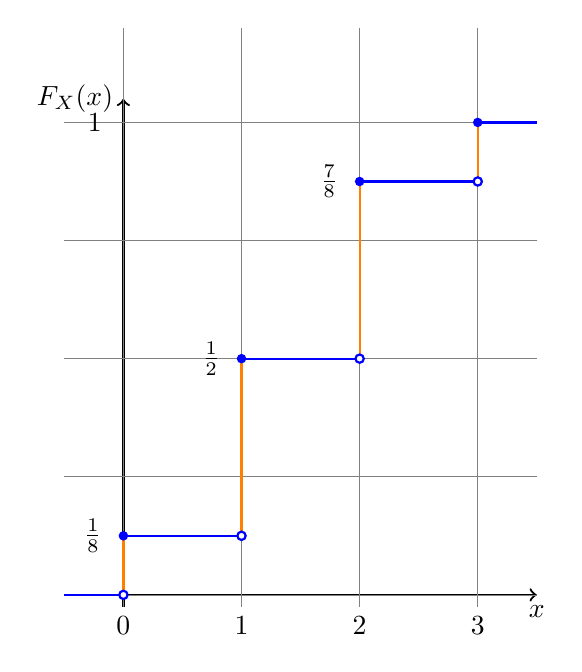
\begin{tikzpicture}[scale=1.5]
    % Define variables for y-coordinates
    \def\yscale{4}
    \def\ya{0.125*\yscale}
    \def\yb{0.5*\yscale}
    \def\yc{0.875*\yscale}
    \def\yd{1*\yscale}

    % Axis
    \draw[thick, ->] (-0.5,0) -- (3.5,0) node[anchor=north] {$x$};
    \draw[thick, ->] (0,-0.1) -- (0,\yscale+0.2) node[anchor=east] {$F_X(x)$};
    \draw[very thin, gray] (-0.5,-0.1) grid (3.5,1.2*\yscale);

    % CDF steps
    \draw[blue, thick] (-0.5, 0) -- (0, 0);
    \draw[orange, thick] (0, 0) -- (0, \ya);
    \draw[blue, thick] (0, \ya) -- (1, \ya);
    \draw[orange, thick] (1, \ya) -- (1, \yb);
    \draw[blue, thick] (1, \yb) -- (2, \yb);
    \draw[orange, thick] (2, \yb) -- (2, \yc);
    \draw[blue, thick] (2, \yc) -- (3, \yc);
    \draw[orange, thick] (3, \yc) -- (3, \yd);
    \draw[blue, thick] (3, \yd) -- (3.5, \yd);

    % Points
    \filldraw[white, draw=blue, thick] (0, 0) circle (1pt);
    \filldraw[blue] (0, \ya) circle (1pt);
    \filldraw[white, draw=blue, thick] (1, \ya) circle (1pt);
    \filldraw[blue] (1, \yb) circle (1pt);
    \filldraw[white, draw=blue, thick] (2, \yb) circle (1pt);
    \filldraw[blue] (2, \yc) circle (1pt);
    \filldraw[white, draw=blue, thick] (3, \yc) circle (1pt);
    \filldraw[blue] (3, \yd) circle (1pt);

    % Labels
    \node at (-0.1, \ya) [anchor=east] {$\frac{1}{8}$};
    \node at (0.9, \yb) [anchor=east] {$\frac{1}{2}$};
    \node at (1.9, \yc) [anchor=east] {$\frac{7}{8}$};
    \node at (-0.1, \yd) [anchor=east] {$1$};
    \node at (0, -0.1) [anchor=north] {$0$};
    \node at (1, -0.1) [anchor=north] {$1$};
    \node at (2, -0.1) [anchor=north] {$2$};
    \node at (3, -0.1) [anchor=north] {$3$};
\end{tikzpicture}
\end{center}
\end{ex}


It is possible to classify all functions that can arise as cumulative distribution functions of random variable as follows:
\begin{thm}[Classification of CDFs]
A function $F(x)$ is a cumulative density function if and only if the following three conditions are satisifies: \begin{enumerate}
\item $\lim_{x\to -\infty}F(x)=0,$  $\lim_{x\to \infty}F(x)=1$
\item $F(x)$ is a non decreasing function
\item $F(x)$ is right continuous. i.e $\lim_{x\to x_o^+}F(x)=F(x_o),$ $\forall x_o\in \R$
\end{enumerate}
\end{thm}


\section{Discrete Random Variables}

\begin{defn}[Discrete Random Variable]
    We say a random variable $X: \mathcal{S} \longrightarrow \mathbb{R}$ is \textbf{discrete} if the cumulative distribution function of $X$, $F_X$ is a step function. 
\end{defn}

\begin{defn}[Probability Mass Function]
    If $X$ is a discrete random variable, the probability mass function associated to $X$ is defined as 
    \begin{eqnarray*}
        p_X :& \mathbb{R} &\longrightarrow \mathbb{R}\\
        & x &\mapsto P(X = x)
    \end{eqnarray*}
    that is, 
    $$p_X(x) := P(\text{$X$ takes the value $x$})$$
\end{defn}
It is easy to observe that the only points where $p_X$ can be non-zero are the values, $\mathcal{X}$, that $X$ can take. 

\begin{defn}[Parameters for Discrete Variables]
Suppose $X$ is a discrete random variable with probability mass function $p_X$ and taking values in the set $\mathcal{X}$. We can consider the following parameters associated to $X$
\begin{enumerate}
    \item \textbf{Expected Value:}
    $$E(X) := \mu_X = \sum_{x\in \mathcal{X}} x\; p_X(x)$$
    \item \textbf{Statisticians Unconscious Law:} Given a function $g: \mathbb{R} \longrightarrow \mathbb{R}$, then 
    $$E(g(X)) := \sum_{x\in \mathcal{X}} g(x) \; p_X(x)$$
    \item \textbf{Variance:}
    \begin{eqnarray*}
        V(X) := \sigma^2_X =& E ((X-\mu_X)^2)\\
        =& \sum_{x\in \mathcal{X}} (x-\mu_X)^2\; p_X(x)
    \end{eqnarray*}
    
\end{enumerate}
    
\end{defn}


\section{Continuous Random Variables}
\begin{defn}[Continuous Random Variable]
We say a random variable $X: \mathcal{S} \longrightarrow \mathbb{R}$ is \textbf{continuous} if the cumulative distribution function of $X$, $F_X$ is a continuous function.
\end{defn}

\begin{defn}[Probability Density Function]
    We say that the function $f_X: \mathbb{R}\longrightarrow \mathbb{R}$ is the probability density function of the continuous random variable $X$ (with cdf $F_X$) if $f_X$ satisfies the following:
    $$ F_X(x) = \int_{-\infty}^x f_X(t) dt$$
\end{defn}

\begin{defn}[Parameters for Continuous Variables]
    Suppose $X$ is a continuous random variable with probability density function $f_X$. We can consider the following parameters associated to $X$
\begin{enumerate}
    \item \textbf{Expected Value:}
    $$E(X) := \mu_X = \int_{-\infty}^\infty x\; f_X(x)\rm{dx}$$
    \item \textbf{Statisticians Unconscious Law:} Given a function $g: \mathbb{R} \longrightarrow \mathbb{R}$, then 
    $$E(g(X))  := \int_{-\infty}^\infty g(x)\; f_X(x)\rm{dx}$$
    \item \textbf{Variance:}
    \begin{eqnarray*}
        V(X) := \sigma^2_X =& E ((X-\mu_X)^2)\\
        =& \int_{-\infty}^\infty (x-\mu_X)^2\; f_X(x)\rm{dx}
    \end{eqnarray*}
\end{enumerate}
\end{defn}


\begin{defn}[Identically Distributed Random Variables]
    We say two random variables $X$ and $Y$ are identically distributed if the corresponding cdfs $F_X$ and $F_Y$ are pointwise equal (almost) everywhere. 
\end{defn}

\begin{ex}
    Suppose we toss a fair coin five times, and $X$ tracks the number of heads in five tosses, and $Y$ tracks the number of tails in five tosses. Then, it is possible to show that even though $X$ and $Y$ are not equal as functions on the sample space, the cdfs $F_X$ and $F_Y$ are exactly the same. As a result $X$ and $Y$ will be identically distributed. 
    \\

    Would we be able to conclude the same if we were to toss an unfair coin?
\end{ex}